\documentclass{article}
\usepackage[margin=1in]{geometry}
\usepackage{../common}
\usepackage{../pagesetup}

\begin{document}
%\lecture{**LECTURE-NUMBER**}{**DATE**}{**LECTURER**}{**SCRIBE**}
\lecture{17}{November 6}{Sasha Rush}{Patrick Varin, Lillian Pentecost, André Snoeck, Baojia Tong, Hsuan Lee}{Loopy BP, Gibbs Sampling, and VI with Gradients}%% Add your scribe names!!

\subsection{Loopy BP}
\subsubsection{History} The history of Loopy Believe Propagation (Loopy-BP) began in 1988 with Judea Pearl who tried to analyze the behavior of the BP algorithm (which gives exact marginal inference on tree) on graphs that are not trees, like the Ising model. Remember the message passing algorithms is
\begin{align*}
	m_{s\to t}(x_t) &= \sum_{x_s}\psi(x_s)\psi(x_s,x_t)\prod_{u\in \text{NBR}(s)-t}m_{u\to s}(x_s)\\
	bel_s(x_s) &\propto \psi(x_s)\prod_{t\in \text{NBR}(s)}m_{t\to s}(x_s)
\end{align*}
Note that this algorithm doesn't require an ordering on the nodes, so it can naturally extend to cyclic graphs.

\FloatBarrier
\begin{figure}
\center
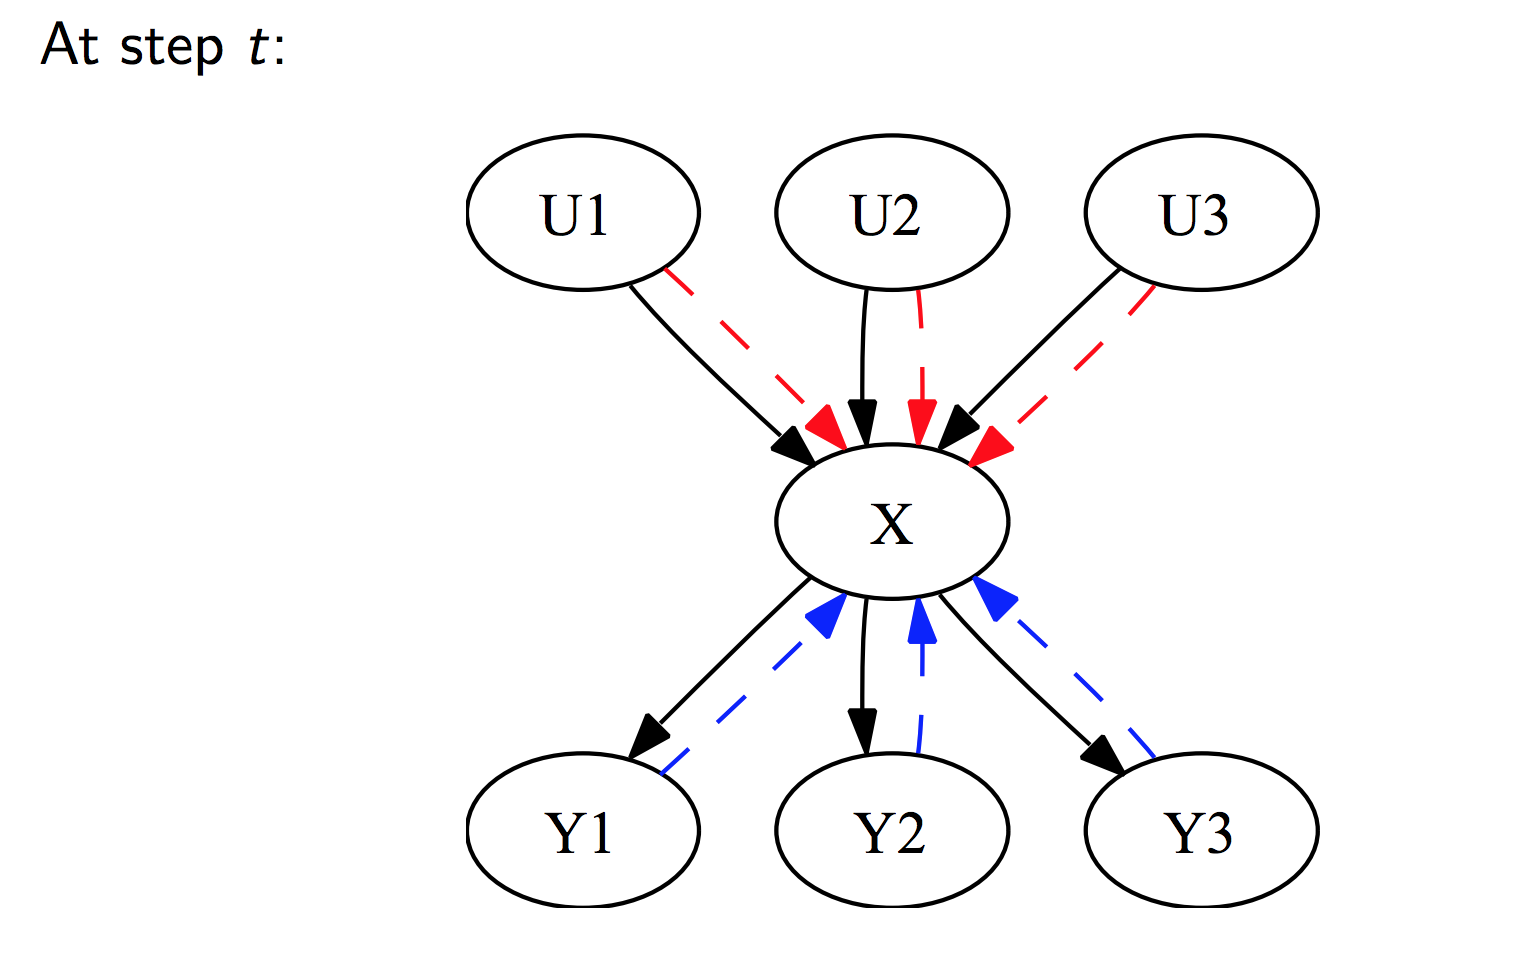
\includegraphics[width=0.4\textwidth]{time_t}
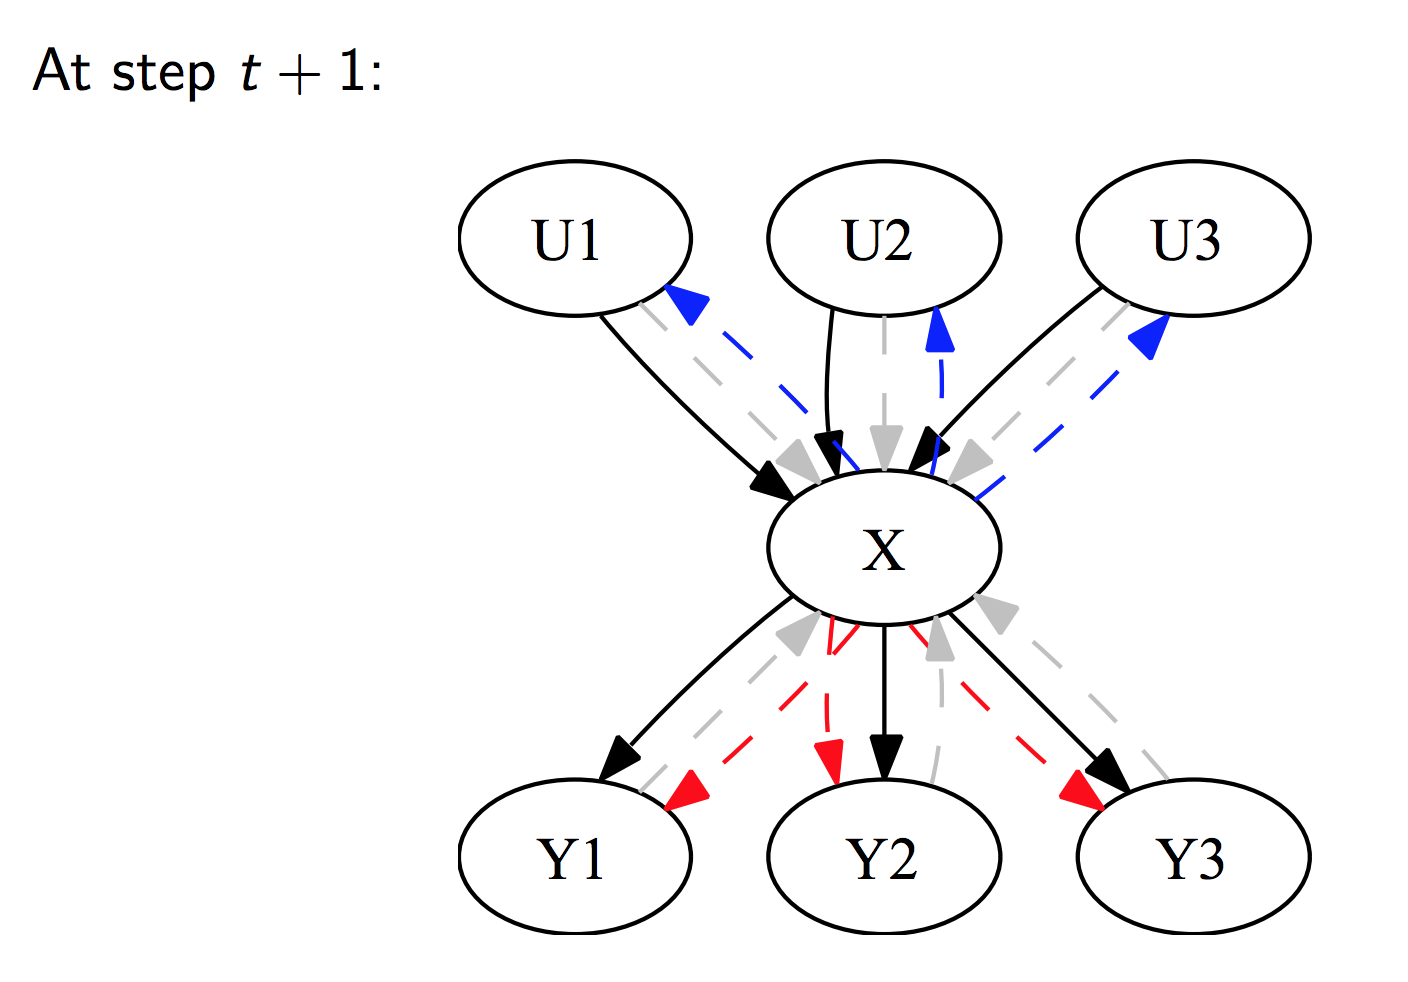
\includegraphics[width=0.4\textwidth]{time_t1}
\caption{Message passing example: left (incoming), right (outgoing)}
\end{figure}

Around 1998, a decade after Pearl raised the question of the BP algorithm on general graphs, papers studying \emph{Turbo coding} or \emph{Low density parity check} (LDPC) codes used the BP algorithm on cyclical graphs with empirical success, motivating more research. This research drew parallels between loopy-BP and variational inference.

\subsubsection{Implementations}
We can implement loopy belief propagation either \emph{synchronously} or \emph{asynchronously}
\begin{itemize}
	\item Synchronous Updates: All of the nodes are updated togethers, so that every node at iteration $t$ depends on it's Markov blanket at $t-1$
	\begin{itemize}
		\item parallelizable
		\item usually takes more updates
	\end{itemize}
	\item Asynchronous Updates: The nodes are given an order and updated sequentially
	\begin{itemize}
		\item sequential
		\item usually converges in fewer updates
	\end{itemize}
\end{itemize}

These updates look similar to mean field variational inference (VI) with some differences in performance.
\begin{itemize}
	\item Loopy BP is exact on trees, mean-field variational inference is not.
	\item Loopy BP is not guaranteed to converge, where VI will.
	\item If Loopy BP converges it is not guaranteed to converge to a local optimum.
\end{itemize}
Loopy BP is generally more costly than mean field VI, because it stores node beliefs in addition to edge messages, whereas mean field VI only stores node parameters. If the graph is large and dense, then Loopy BP might be very costly. 

In practice, because Loopy BP contains more information about the problem than mean field VI it tends to work better.

\subsection{Gibbs Sampling (Preview)}

Gibbs Sampling is a different method for approximate inference. It is a special case of Markov Chain Monte Carlo (MCMC), which will be covered in more detail in coming lectures. 

The main idea of Gibbs Sampling is to re-estimate the posteriors for $x_i$ assuming that we have we have explicit point estimates for all the other nodes in the graph ($x_{-i}$):

$$\tilde{x}_i \sim P(x_{i} | \tilde{x}_{-i})$$

Naturally, we only care about the Markov blanket when estimating a particular node. Gibbs sampling is not a parallel algorithm, the samples have to be generated sequentially. However, we can go through our graph in any particular order and update each node accordingly. 

\subsubsection{Example: Gibbs Sampling Topic Modeling}

In the following example, we present the Gibbs update associated to the topic modeling that we defined in Lecture 16. Remember that 

\begin{align*}
\beta_k \sim Dir(\eta)& &k\text{ topics} \\
\pi_n \sim Dir(\alpha)& &n\text{ documents} \\
z_{ni} \sim Cat(\pi_n)& &\text{Draw topic for each word and each document} \\
w_{ni} \sim Dir(\beta_{z_{ni	}})& &\text{Draw a word from a topic} \\
\end{align*}

and the full joint distribution is given by 

% Use \pi instead of \theta
\begin{equation*}
p(\beta_k, \pi_n, \{z\}, \{w\}) = \prod_{k}{p(\beta_k)}\prod_{n}{p(\pi_n)}\prod_{n,i}{p(z_{ni} | \pi_n){p(w_{ni} | z_{ni})}}
\end{equation*}

See Figure \ref{fig:topic_modeling} for reference. 

\begin{figure}[!ht]
\centering
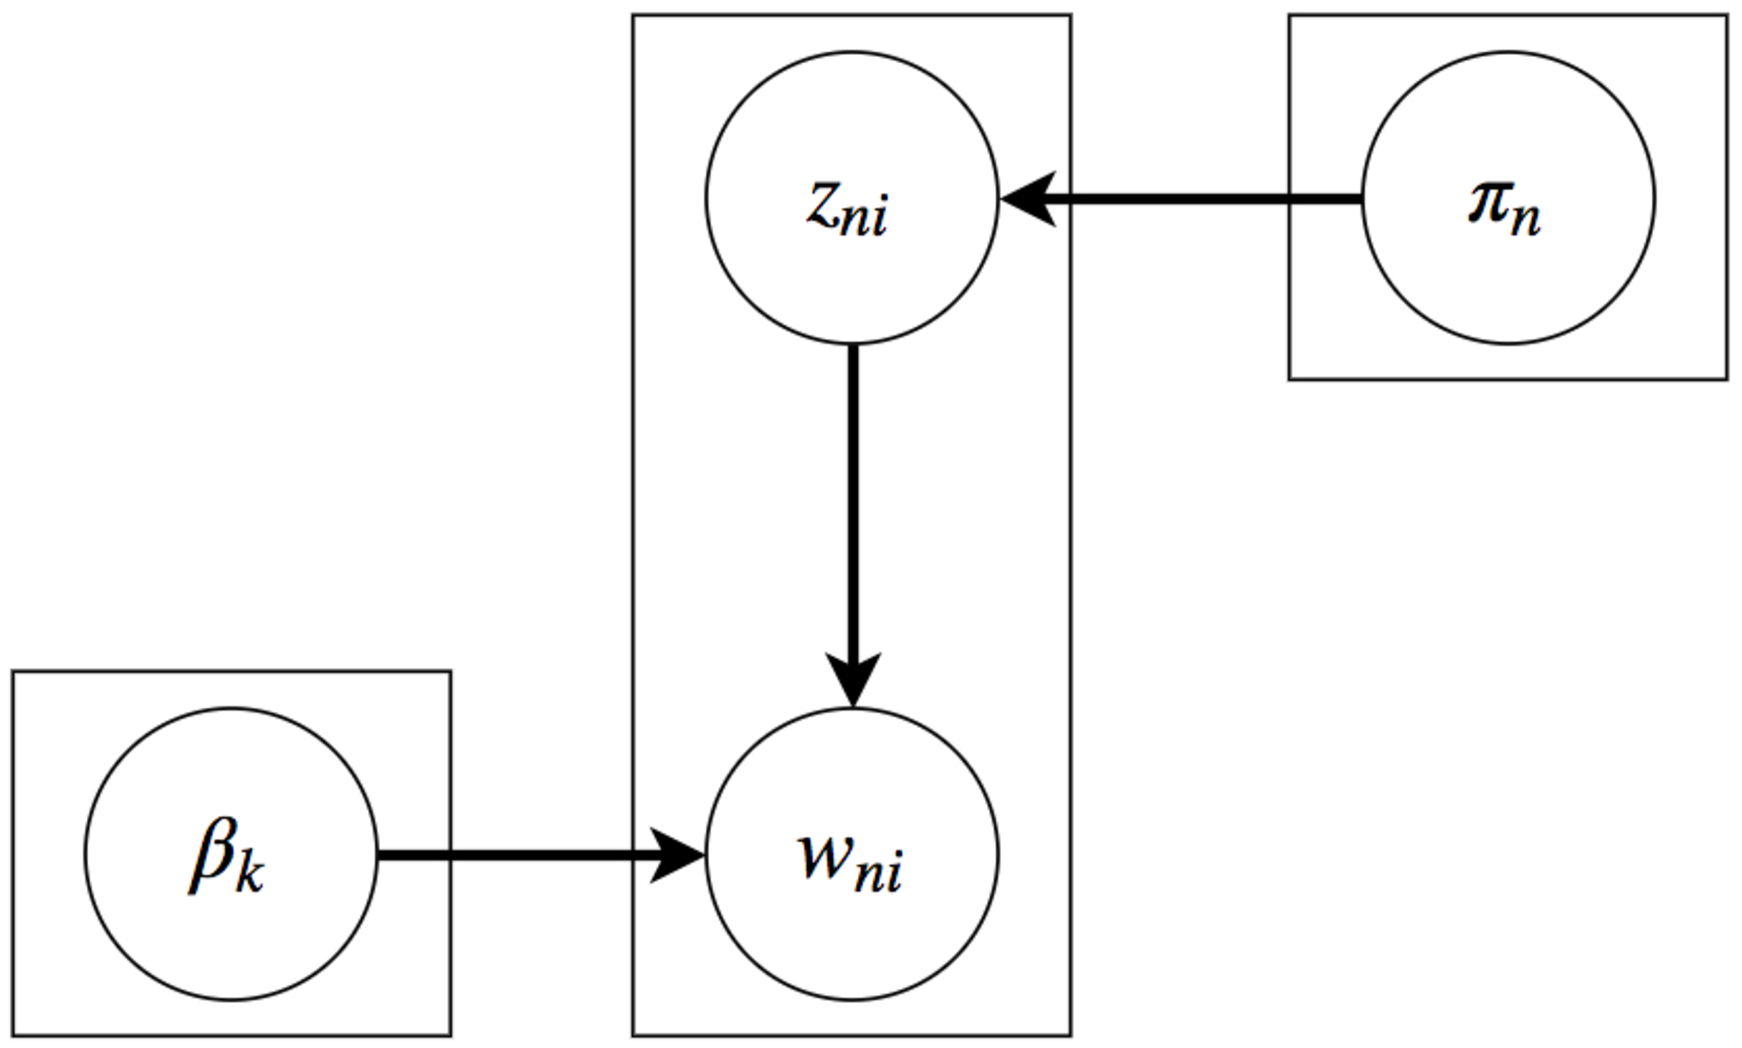
\includegraphics[width = 0.4\textwidth]{topic_model.pdf}
%\vspace{-0.2cm}
\caption{Graphical model associated to topic modeling example}
\label{fig:topic_modeling}
%\vspace{-0.5cm}
\end{figure}

% \begin{equation*}
% p(\beta_k, \theta_n, \{z\}, \{w\}) = \prod_{k}{p(\beta_k)}\prod_{n}{p(\theta_n)}\prod_{n,i}{p(z_{ni} | \theta_n){p(w_{ni} | z_{ni})}}
% \end{equation*}

The updates for Gibbs sampling are similar to those of Mean Field (see Lecture 16), albeit much simpler. We need to compute the conditional probability for each of the following

\begin{align*}
z_{ni} = k | \pi_n, w_{ni} &\propto \pi_{nk}\beta_{k,w_{ni}} \\
\pi_n | \alpha, z_{ni} &= Dir(a_k + \sum_{i}\mathbb{1}(z_{ni} = k)) \\
\beta_k = d | \eta, z_{ni} &= Dir(\eta_d + \sum_{i}\mathbb{1}(z_{ni} = k, w_{ni} = d))
\end{align*}

The last two terms are essentially the full posterior that we saw in lecture 2. Although these updates are rather simple, it is used in many applications given it works with a wide variety of models. Typically, one would draw one sample per update. It is not clear whether drawing multiple samples or running more epochs helps the algorithm converge faster. 

\subsection{Variational Inference with Gradients}

\subsubsection{Introduction}
Variational inference with gradients is also referred to as black box variational inference or stochastic variational inference (SVI) and is actively gaining traction in the ML commnity today.  
For example, UberAI just released a new framework on top of pytorch called \textit{pyro} to support SVI.  
One reason why this is attractive is because SVI integrates well with autograd and deep learning.


\subsubsection{Aside on Monte Carlo Sampling}

If we consider some expectation over a distribution $p$ of some function $f(z)$, as given below for discrete $z$, we often find this is intractable to compute.

$$
\E_{z \sim p}[f(z)] = \sum_{z'} p(z') f(z')
$$

We can approximate this expectation by sampling some $N$ number of $\tilde{z}$, with each sample represented by $\tilde{z}_n$, which results in the following expression for the expectation:

$$
\E_{z \sim p}[f(z)] \approx \frac{1}{N} \sum_{n=1}^{N} f(\tilde{z}_n)
$$

This is much simpler to compute, and it can be shown that the resulting $\tilde{\mu}$ satisfies that $(\tilde{\mu}- \mu) \sim \N(0, \frac{\sigma^2}{N})$, which implies that the variance of the approximation with respect to the true mean decreases with the number of samples $N$.

\subsubsection{Rough Idea}

We will apply gradient optimization to the lower bound on $p(x)$ that we use to derive the variational objective.  
We use the formulation of the Gaussian Mixture Model (GMM) and Mean Field (MF) approximation with variational parameters, developed in previous lectures, as an example.  
This is potentially more attractive than coordinate ascent because for a very large dataset compared to the number of classes (i.e. $n >> k$ in the GMM MF configuration) coordinate ascent requires (1) iterating through all data to perform updates to the variational parameters and (2) storing variational parameters per-example (the number of the parameters grows with the size of the dataset).


The two wishes/ideas of this approach will be to (1) update global parameters ($\lambda_k$) on mini-batches to avoid the need to iterate over all samples (all $\lambda_n$) to perform update and (2) avoid storage of a dedicated $\lambda_n$ for each $n$.
The remainder of the lecture will focus on idea (1) above.


\subsubsection{Deriving the Variational Objective}

Letting $\theta = {z_n, \mu_k}$, we would like $p(x)$ for the GMM MF configuration previously developed.  
We aim to maximize the following lower bound (also from previous lecture) in order to approach $p(x)$, where $q_{\lambda}$ is any $q$ with variational parameters $\lambda$.

$$
p(x) \geq \E_q [\log{\frac{p(x, \theta)}{q_{\lambda}(\theta)}} ]
$$

$$
\max_{q} \E_q [\log{\frac{p(x, \theta)}{q_{\lambda}(\theta)}} ]
$$

Expressing $p(x, \theta) = p(\theta) p(x|\theta)$ and distributing the log, we find the variational objective, and we can interpret each of the three terms:

$$
\max_{q} - \E_q [\log{q_{\lambda}(\theta)} ] + \E_q [\log{p(\theta)} ] + \E_q [\log{p(x|\theta)} ]
$$

In the expression above, we can recognize that the first term is just an entropy term, the second term includes the prior to effectively find a $q$ close to $p(\theta)$ based on cross-entropy, and the third term contains the likelihood to reflect how well $\theta$ predicts the data.  
Furthermore, we see that the first two terms together form the negative inverse KL divergence of $p$ and $q$, so we further simplify to the expression below:

$$
L(\lambda) = \max_{q} - KL(q(\theta) || p(\theta)) + \E_q (\log{p(x|\theta)})
$$

In the expression above, the KL divergence will act to tend $q$ towards the prior $p(\theta)$ and the expectation term will give weight in $q$ to parameters that tend to explain $x$.

\subsubsection{Optimization via Stochastic Gradient Descent (SGD)}

Next, we aim to apply optimization via SGD, and the $L(\lambda)$ given above becomes a loss function; we will maximize the value of this function by computing the gradient with respect to the parameters we care about ($\lambda$).  
Here, we will take a mini-batch of $x$ values and compute $\nabla_{\lambda} L(\lambda)$.  
However, we notice that the expectation term in $L(\lambda)$ over $q$ must be approximated, and the two methods to compute an approximation are (1) reinforcement and (2) reparameterization.
This lecture only covers method (2), reparameterization, which also appears on HW4.

Reparameterization requires known $q$ of a certain type and removes q from the expectation.  
Beginning with the form of the expectation, we can reformulate in terms of a change of variable from distribution q to the standard normal (letting $\theta = Az+b$) and then apply the Monte Carlo approximation to simplify the expression and make it computationally tractable:

$$
\E_{q_{\lambda}} [p(x|\theta)] = \E_{z \sim \N(0,1)} [p(x|f_{\lambda}(z))]
$$

$$
\nabla_{\lambda} \E_{z \sim \N(0,1)} [p(x|f_{\lambda}(z))] = \E_{z \sim \N(0,1)} [ \nabla_{\lambda} p(x|f_{\lambda}(z))]
$$

$$
\nabla_{\lambda} \E_{q_{\lambda}} [p(x|\theta)] \approx \frac{1}{N} \sum_{n=1}^{N} \nabla_{\lambda} p(x|f_{\lambda}(\tilde{z}_n))
$$
\end{document}
